% !TEX root = ../main.tex

% 分析与讨论	
\begin{table}
	\renewcommand\arraystretch{1.7}
	\begin{tabularx}{\textwidth}{|X|X|X|X|}
		\hline
		Major：& Physics &Grade：& 2022\\
		\hline
		Name： & 杨舒云 & Student number：& 22344020\\
		\hline
		Date：& 2024/12/30 & Score： &\\
		\hline
	\end{tabularx}
\end{table}
\section{APL1-2 Vacuum Compatibility Testing of Materials and Plasma Characteristics Study \\ Analysis \& Discussion}


%---------------------------------------------------------------------
% 数据处理
\subsection{Data Processing}

% 分析
\subsubsection{Analysis}
\begin{enumerate}
	\item 通过真空气体放电实验， 测量击穿电压与电极间隙和气压之间的关系， 验证帕邢定律， 了解气体放电基本物理过程。
	
	根据Paschen定律，考虑采用函数$V_d=\frac{Ap}{\ln (Bp)}$进行拟合，拟合结果如\cref{fig:apl12exp22}所示。
	
	\begin{figure}[htbp]
		\centering
		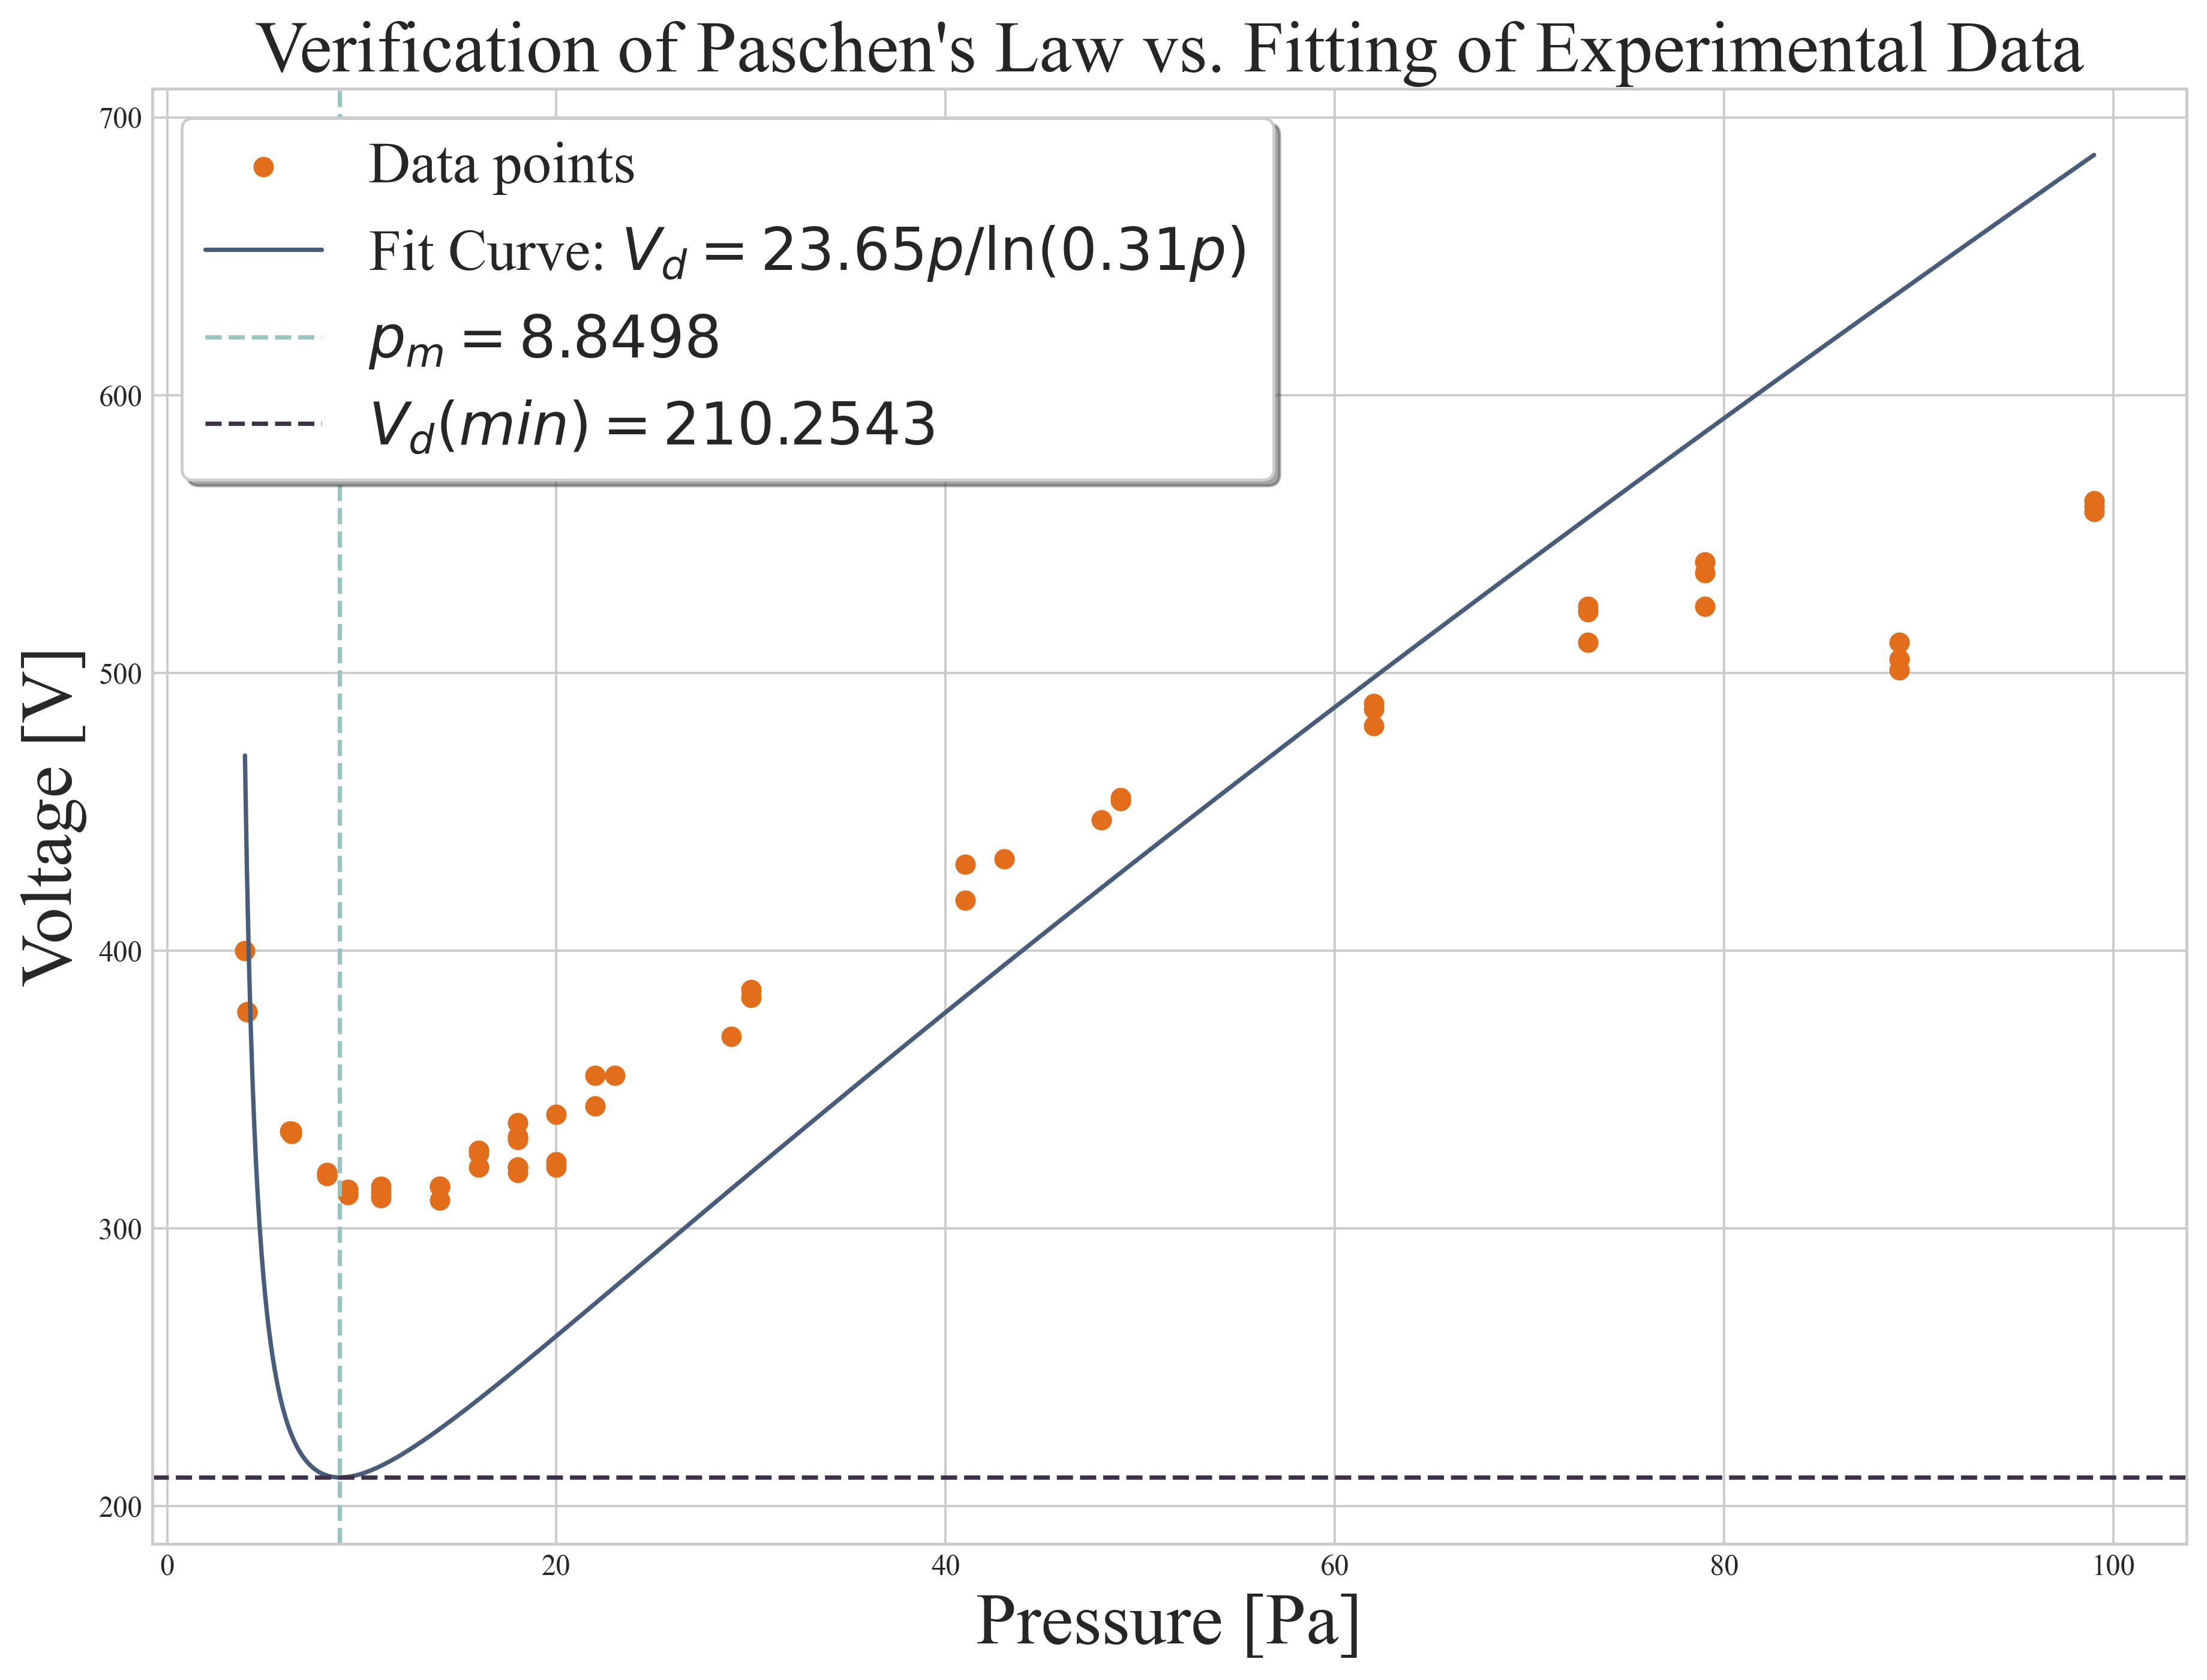
\includegraphics[width=0.7\linewidth]{images/APL1_2_exp2_2}
		\caption{击穿电压-压强关系（拟合）}
		\label{fig:apl12exp22}
	\end{figure}
	
	从拟合结果看出，实验结果基本验证了Paschen定律。
	
	\item 测定了 Ar 气体放电产生的等离子体光谱后，可以通过以下方法分别求解电子温度 (\(T_e\))、电子密度 (\(n_e\)) 和离子密度 (\(n_i\))。
	
	电子温度 (\(T_e\)) 反映了等离子体中自由电子的平均能量，可以通过谱线强度比法 (Boltzmann Plot Method) 或两谱线强度比法求解。在 Boltzmann 图法中，利用公式：
	\[
	\ln\left(\frac{I_{ij} \lambda_{ij}}{g_i A_{ij}}\right) = -\frac{E_i}{k_B T_e} + \ln\left(\frac{hc N}{Z(T)}\right)
	\]
	其中，\(I_{ij}\) 是谱线强度，\(\lambda_{ij}\) 是谱线波长，\(g_i\) 是能级的简并度，\(A_{ij}\) 是自发辐射跃迁几率，\(E_i\) 是上能级能量，\(Z(T)\) 是配分函数，\(k_B\) 是玻尔兹曼常数，\(h\) 是普朗克常数，\(c\) 是光速。选择多个高能跃迁谱线，记录其强度和波长，查表获取对应的 \(\{E_i, g_i, A_{ij}\}\)，绘制 \(\ln(I_{ij} \lambda_{ij} / g_i A_{ij})\) 对 \(E_i\) 的关系图，斜率为 \(-1 / (k_B T_e)\)。或通过两谱线强度比公式：
	\[
	\frac{I_1}{I_2} = \frac{g_1 A_1}{g_2 A_2} \exp\left(-\frac{E_1 - E_2}{k_B T_e}\right)
	\]
	选取两条已知能级差的谱线，通过强度比直接求解 \(T_e\)。
	
	电子密度 (\(n_e\)) 通常通过谱线加宽效应，特别是斯塔克加宽来测定。斯塔克加宽公式为：
	\[
	\Delta\lambda_{Stark} = 2w \cdot n_e^{2/3}
	\]
	其中，\(\Delta\lambda_{Stark}\) 是谱线的斯塔克加宽（半高全宽，FWHM），\(w\) 是与谱线跃迁相关的斯塔克加宽参数。选择无显著自吸效应的谱线，测量其半高全宽 \(\Delta\lambda_{Stark}\)，结合查表所得的 \(w\) 值，通过公式反推出 \(n_e\)。若存在显著自由-自由或自由-束缚辐射，也可利用背景辐射强度与电子密度的关系推导 \(n_e\)。
	
	离子密度 (\(n_i\)) 则通过电离平衡条件结合电子温度和电子密度推算，常用萨哈方程：
	\[
	\frac{n_{i+1} n_e}{n_i} = \frac{2Z_{i+1}}{Z_i} \left(\frac{2\pi m_e k_B T_e}{h^2}\right)^{3/2} \exp\left(-\frac{E_{ion}}{k_B T_e}\right)
	\]
	其中，\(n_i, n_{i+1}\) 是离子化前后离子的密度，\(Z_i, Z_{i+1}\) 是配分函数，\(E_{ion}\) 是电离能，\(m_e\) 是电子质量。结合光谱中离子谱线强度和已知的 \(T_e\)、\(n_e\)，可迭代计算 \(n_i\)。此外，还可以通过谱线相对强度结合配分函数和电离能参数推导离子密度。
	
	然而，由于实验室Ar与Ne均不纯，He相对纯净，以下以He给出上述分析的示例。
	\begin{enumerate}
		\item \textbf{光谱测量数据}：
		\begin{itemize}
			\item 主峰位置：$501.099 \, \mathrm{nm}$
			\item 主峰强度：$521.0 \, \mathrm{arb. \, units}$
			\item 半高全宽 (FWHM)：$1.1545 \, \mathrm{nm}$
		\end{itemize}
		
		\item \textbf{电子温度 ($T_e$)}：使用 Boltzmann 图法，选取氦光谱线 ($587.244 \, \mathrm{nm}, 667.311 \, \mathrm{nm}, 501.099 \, \mathrm{nm}$) 的能级信息，计算得到：
		\[
		T_e = 0.94 \, \mathrm{eV}
		\]
		
		\begin{figure}[htbp]
			\centering
			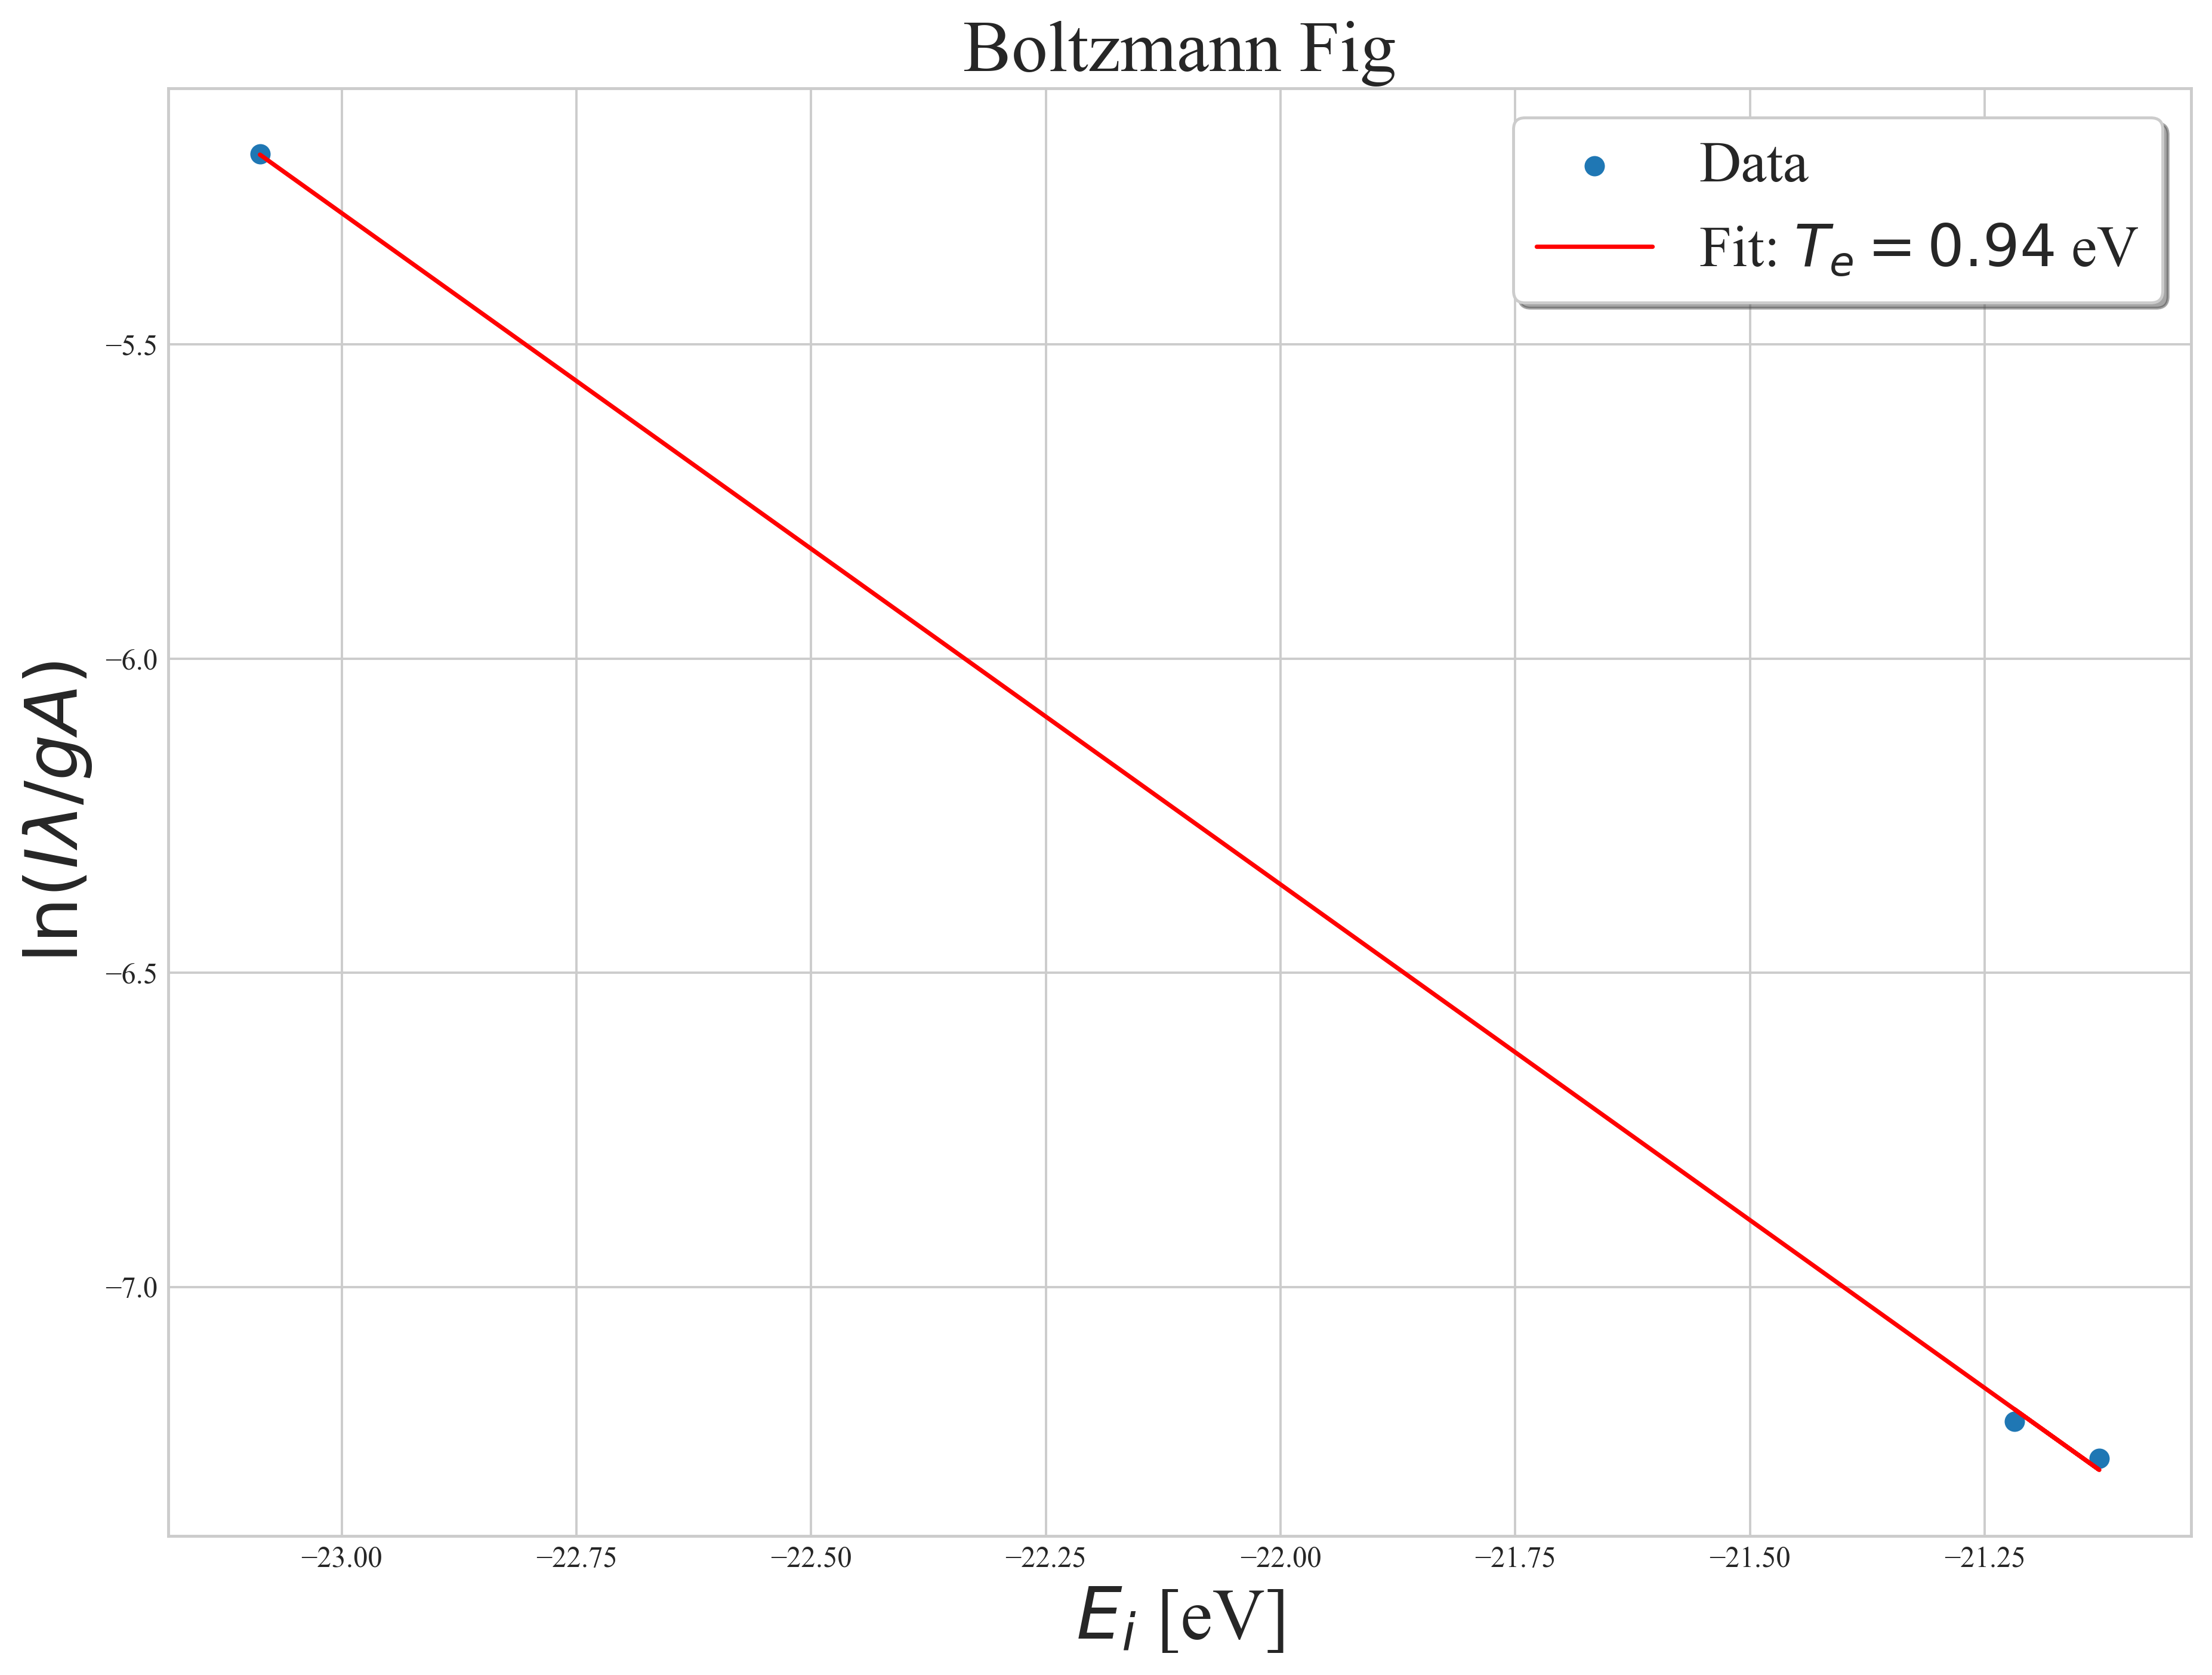
\includegraphics[width=0.7\linewidth]{images/APL1_2_exp3_BF}
			\caption{He-Boltzmann 图}
			\label{fig:apl12exp3bf}
		\end{figure}
		
		\item \textbf{电子密度 ($n_e$)}：基于主峰 ($501.099 \, \mathrm{nm}$) 的半高全宽 ($1.1545 \, \mathrm{nm}$) 和斯塔克加宽参数 ($w = 0.05 \, \mathrm{nm \cdot cm^3}$)，计算得到：
		\[
		n_e = 2.71 \times 10^{19} \, \mathrm{cm^{-3}}
		\]
		
		\item \textbf{离子密度 ($n_i$)}：假设总粒子密度 $n_{\text{total}} = 1 \times 10^{19} \, \mathrm{cm^{-3}}$，基于萨哈方程计算得：
		\[
		n_i \approx 9.99 \times 10^{18} \, \mathrm{cm^{-3}}, \quad n_{i+1} \approx 3.21 \times 10^{13} \, \mathrm{cm^{-3}}
		\]
	\end{enumerate}	
	
	\item 质谱仪谱线分析，考虑扣除如\cref{fig:apl124bg}所示本底。
	
	\begin{figure}[htbp]
		\centering
		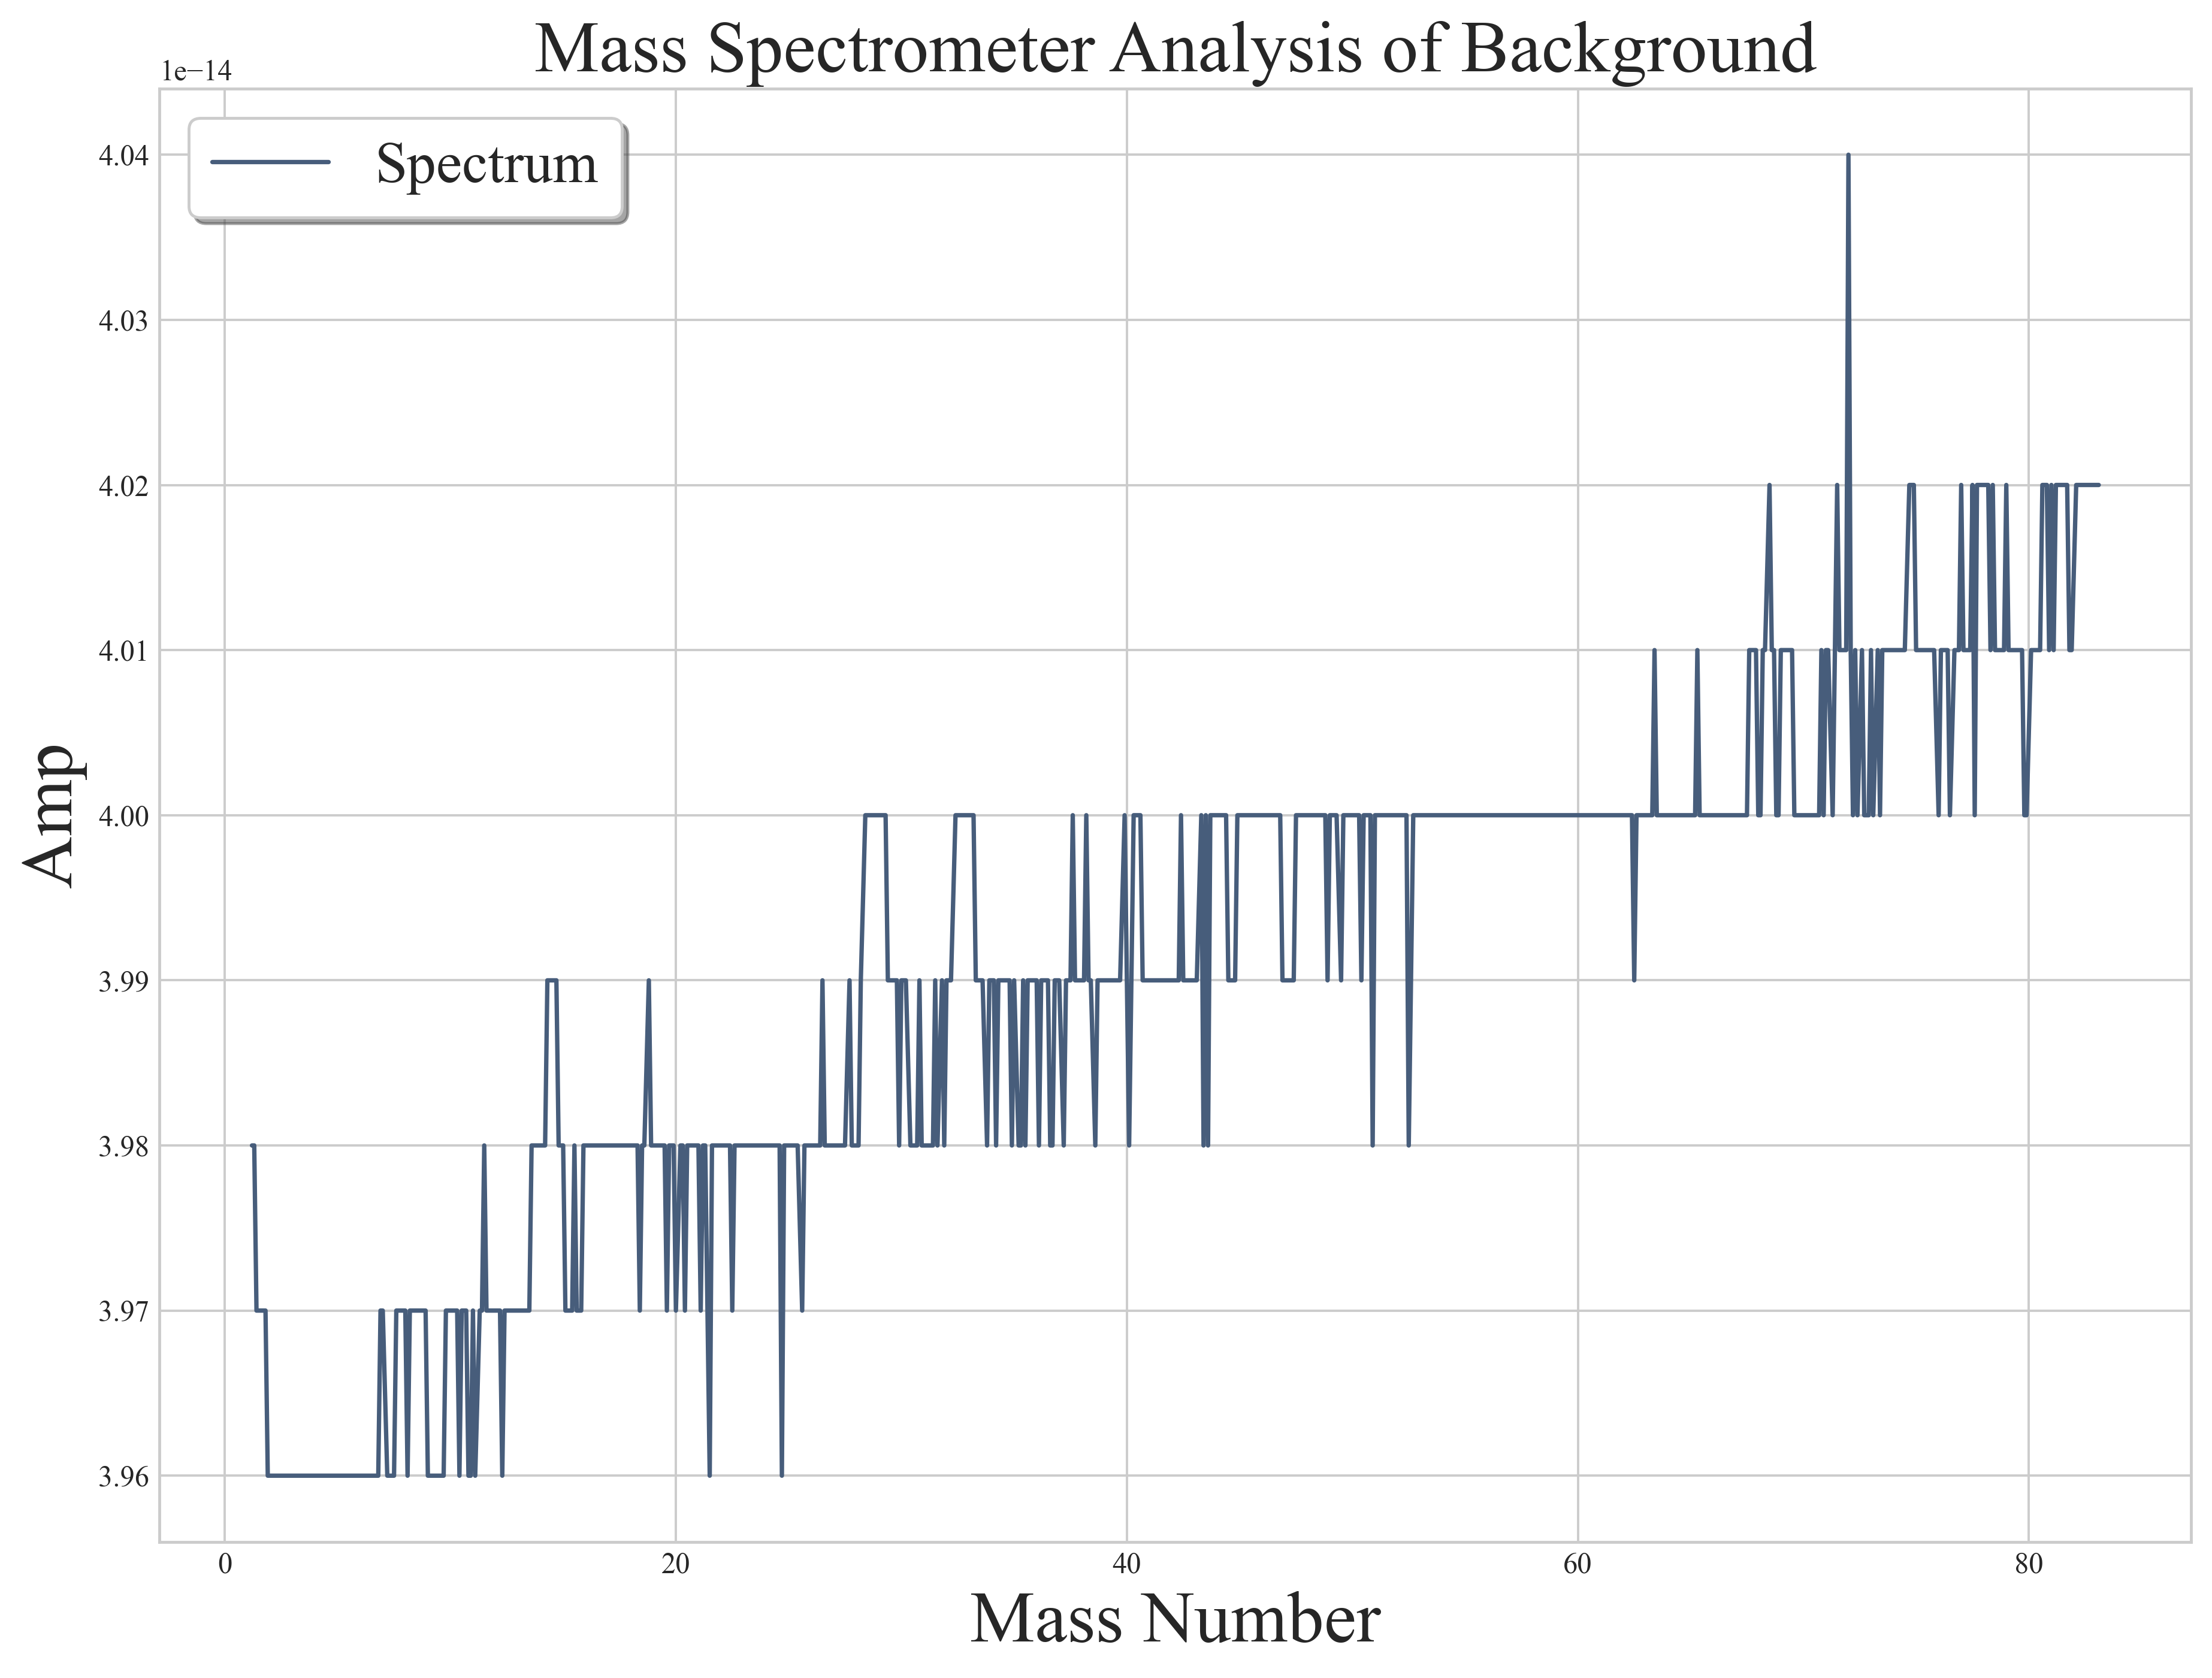
\includegraphics[width=0.7\linewidth]{images/APL1_2_4_bg}
		\caption{质谱仪背景}
		\label{fig:apl124bg}
	\end{figure}
	
	然后利用寻峰算法寻找主要谱线，结果见讨论部分。
	
\end{enumerate}

% 讨论
\subsubsection{Discussion}
\begin{enumerate}
	\item 基于He放电光谱讨论其等离子体参数特性
	\begin{enumerate}
		\item 测定了氦气放电等离子体的关键参数，包括电子温度 ($T_e = 0.94 \, \mathrm{eV}$) 和电子密度 ($n_e = 2.71 \times 10^{19} \, \mathrm{cm^{-3}}$)，表明该等离子体具有典型的低温高密度特性。离子密度 ($n_i$) 显著高于一次电离态 ($n_{i+1}$) 的密度，符合氦气高电离能的特性。
		\item 等离子体主要由中性粒子和少量一次电离的离子组成，电子与离子的相互作用主导了其光谱特性。电子密度较高，表明等离子体中存在显著的碰撞过程。
		\item Boltzmann 图法和斯塔克加宽法提供了可靠的参数估算手段，
		结合萨哈方程进一步拓展了对离子分布的理解。
	\end{enumerate}
	
	\item 质谱仪测定结果讨论
	\begin{enumerate}
		\item 空气
		\begin{itemize}
			\item 质量数 14.4 和 28.7：质量数约为 14.4 的峰可能对应于 N+（氮原子离子）。质量数约为 28.7 的峰可能对应于 N2+（氮气分子离子），氮气占空气的主要组成部分（~78\%）。
			\item 质量数 32.6：质量数约为 32.6 的峰可能对应于 O2+（氧气分子离子）。氧气是空气的第二大成分（~21\%）。
			\item 其他小峰：小峰可能对应于少量的稀有气体（如氩 Ar）或其他痕量成分（如 CO2、H2O）。
		\end{itemize}
		
		\begin{figure}[htbp]
			\centering
			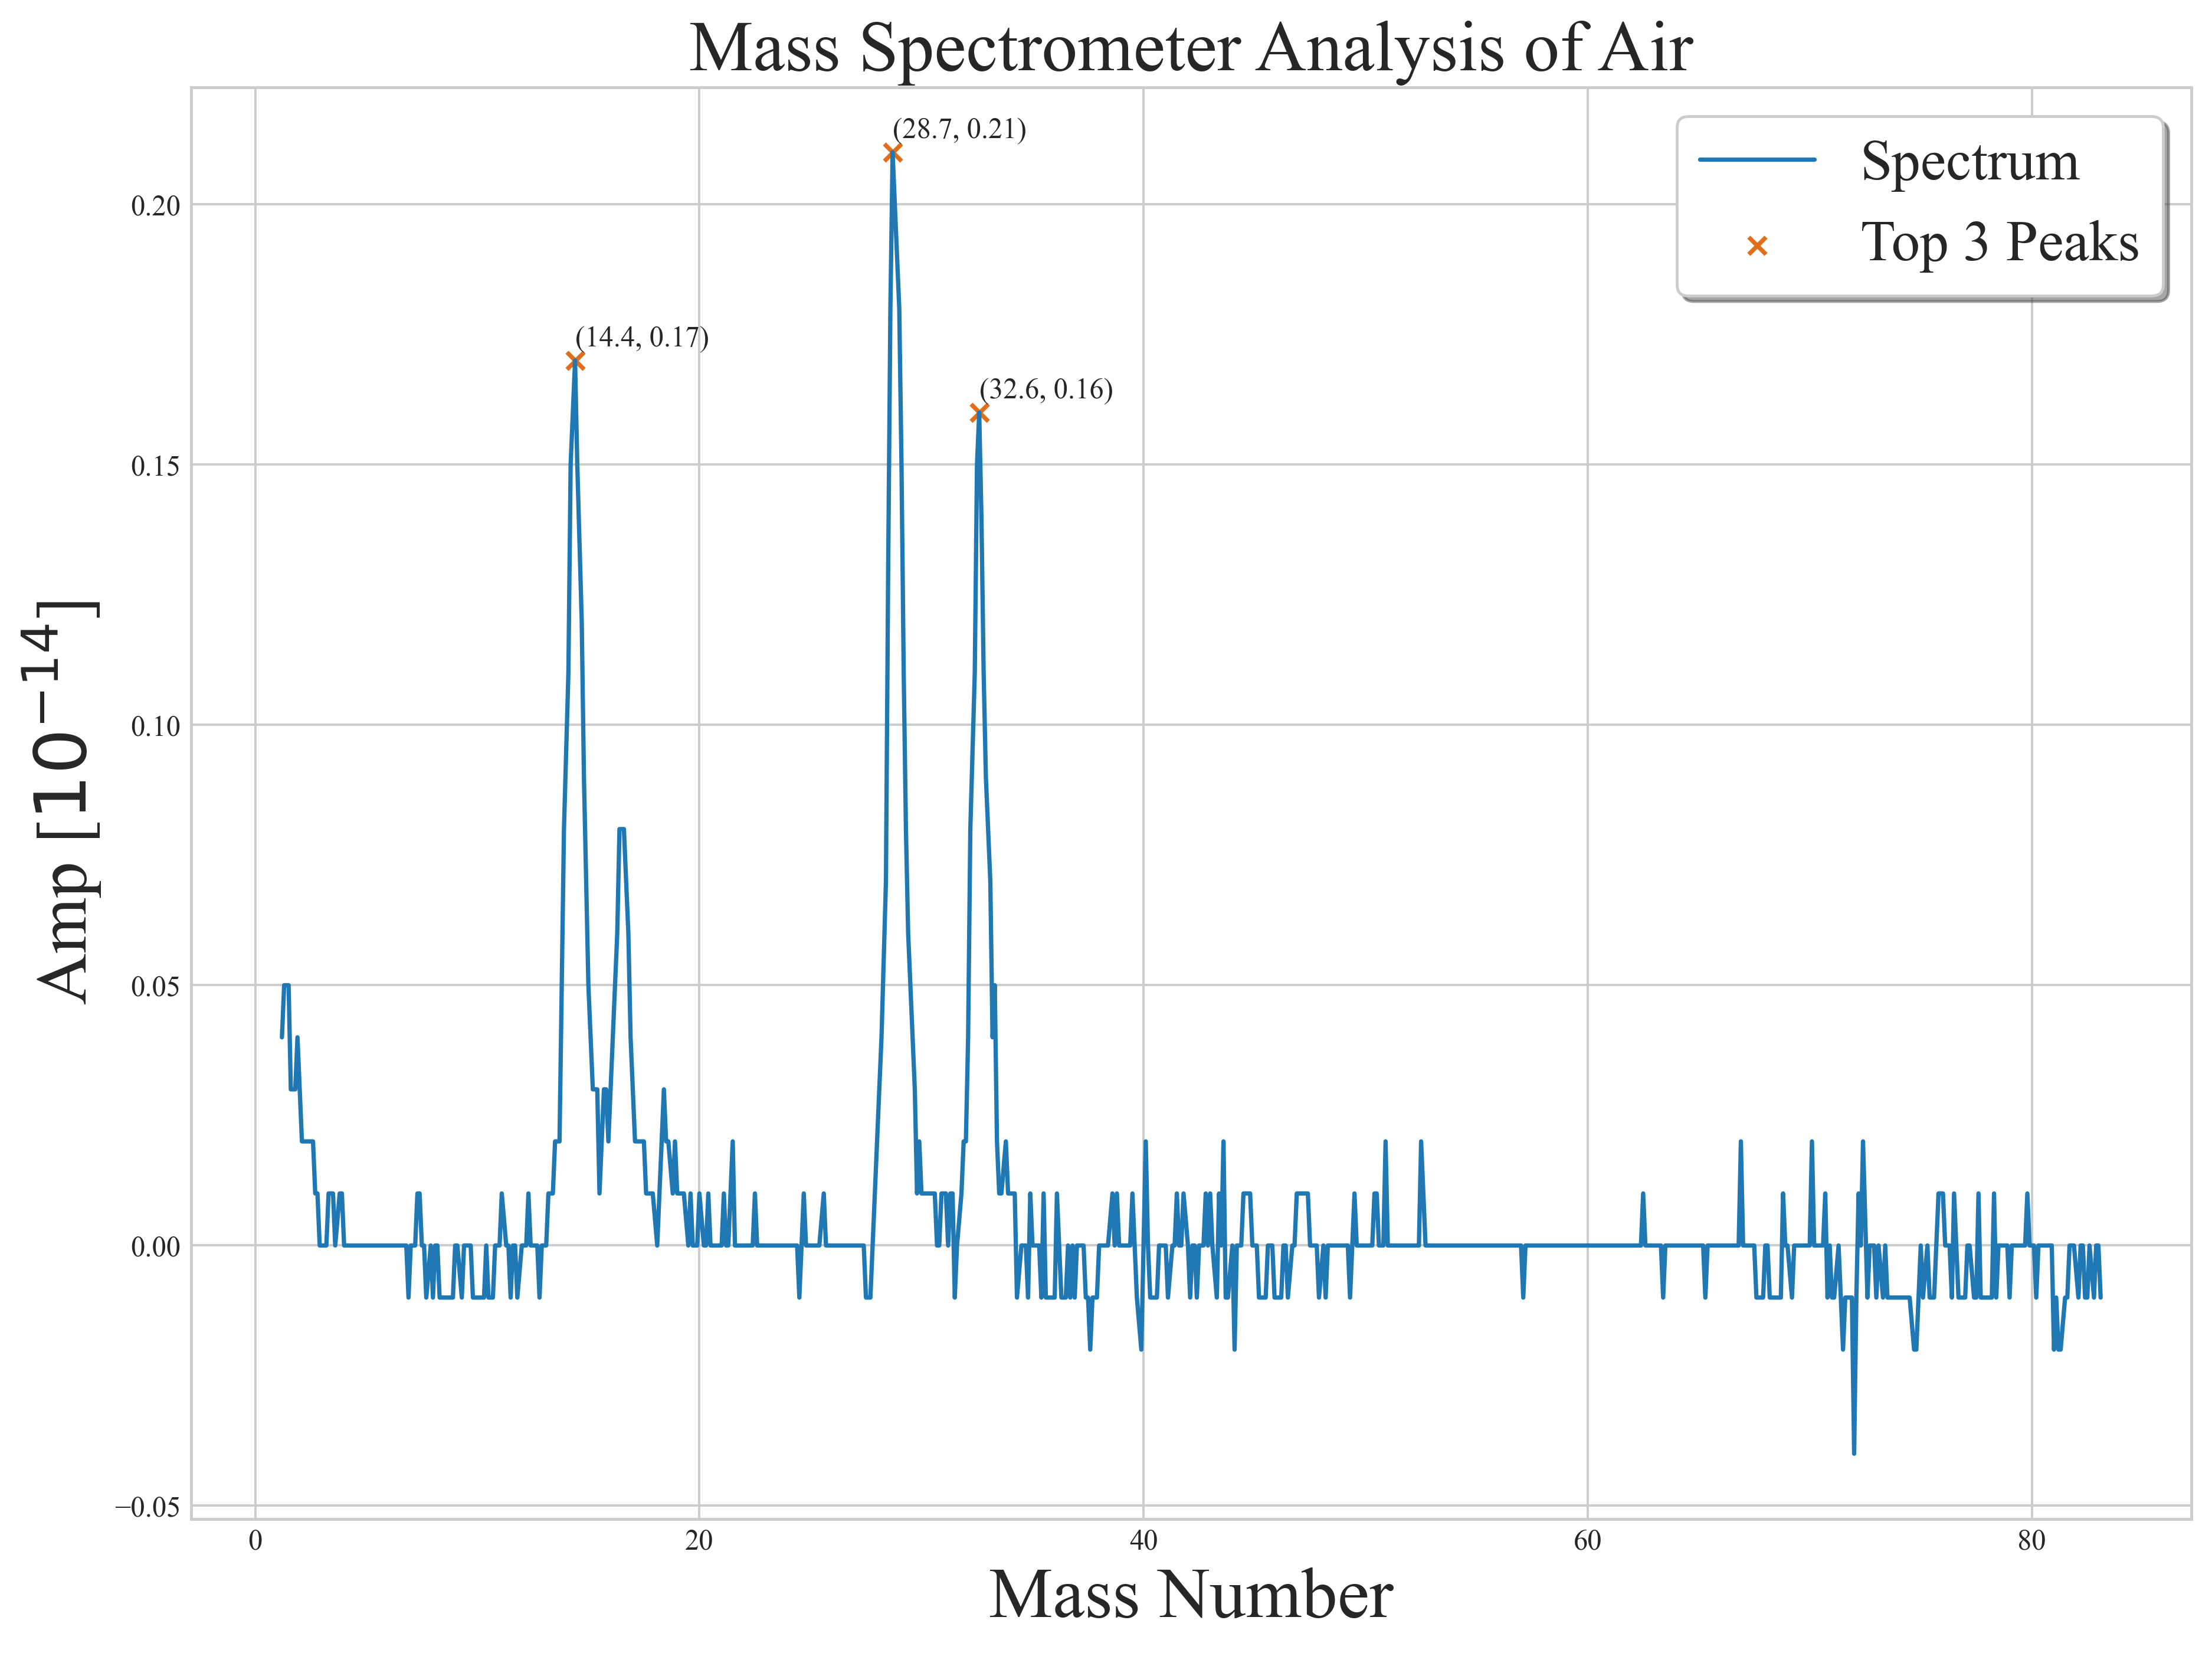
\includegraphics[width=0.7\linewidth]{images/APL1_2_4_air}
			\caption{空气的质谱仪谱线分析}
			\label{fig:apl124air}
		\end{figure}
		
		\item Ar
		\begin{itemize}
			\item 质量数 40.7：这是 Ar 的主要同位素 40Ar 的离子峰。氩气的主要同位素是 40Ar，占比约 99.6\%，因此这是谱图中最显著的峰。
			\item 质量数 20.6 和 18.5：这些可能是仪器背景噪声或少量氩气中的其他同位素贡献，如 36Ar 或 38Ar，但信号偏低可能也与质谱仪的检测灵敏度和分辨率有关。
			
			20.6还有一种更有可能的结果：40Ar的二价离子（电荷数为2）。
			
			18.5 的峰可能是水分子（H2O）的背景信号，因为实验环境中的水蒸气常见于质谱背景。
		\end{itemize}
		
		\begin{figure}[htbp]
			\centering
			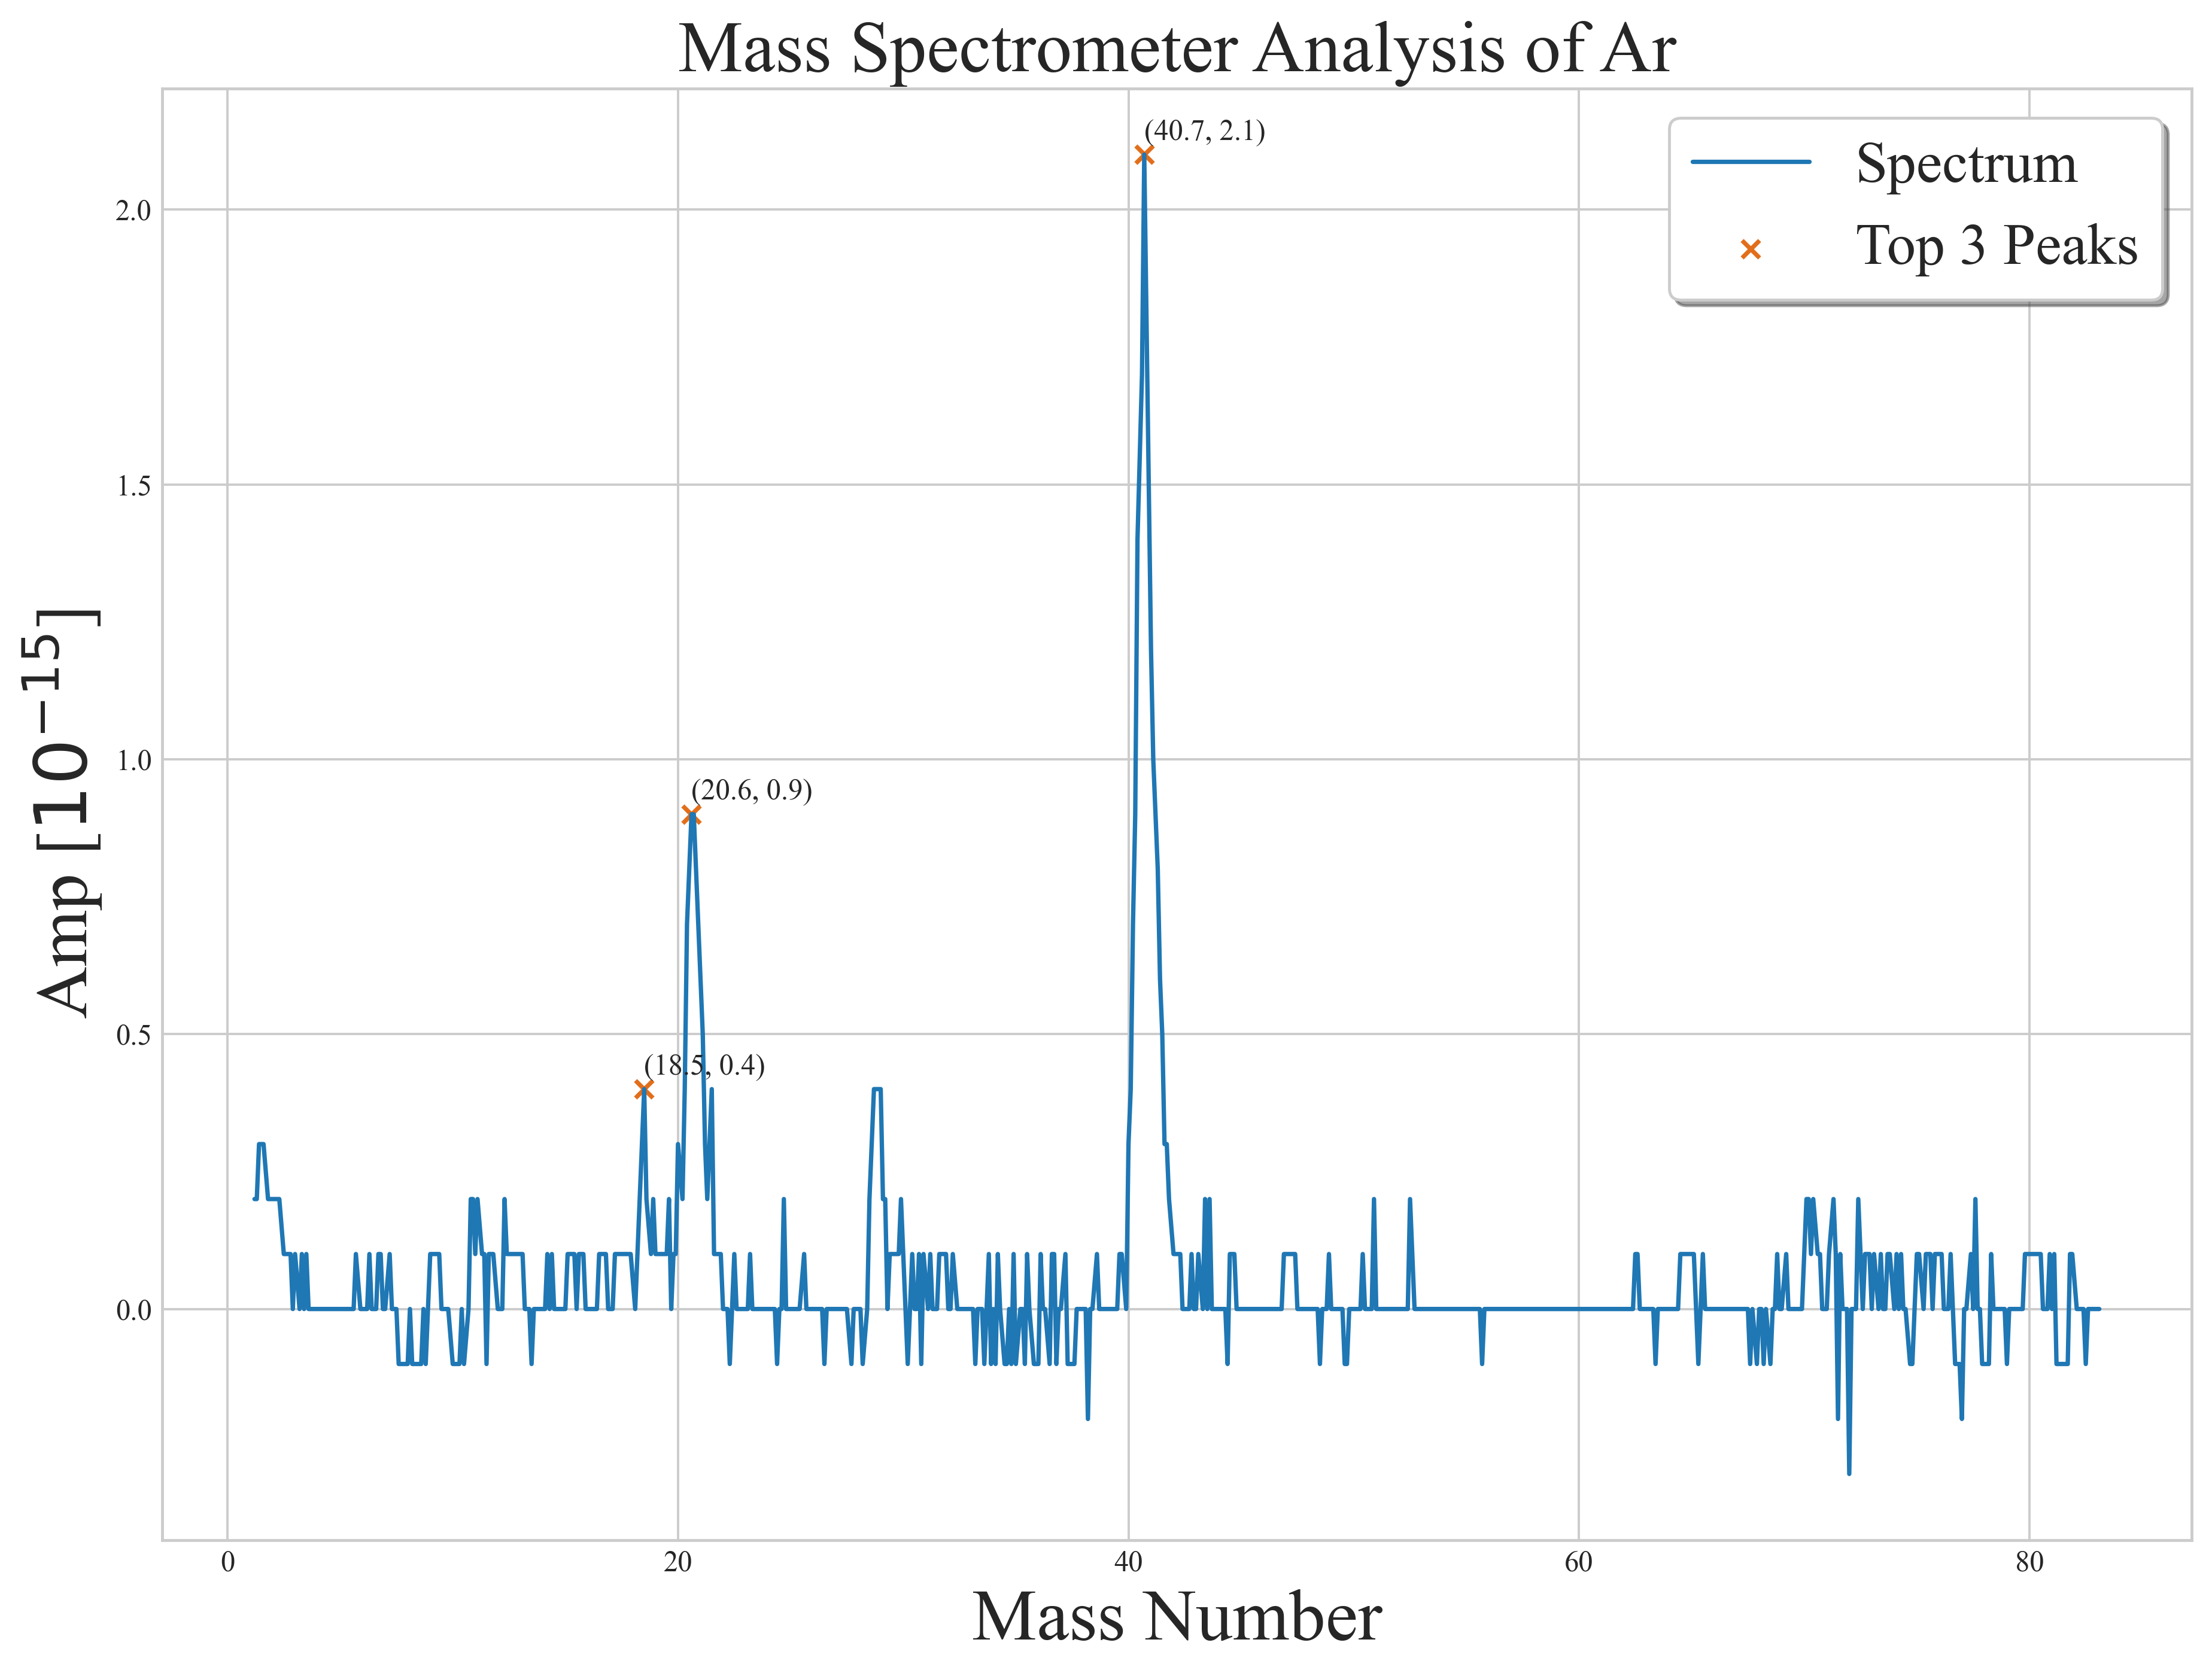
\includegraphics[width=0.7\linewidth]{images/APL1_2_4_Ar}
			\caption{Ar的质谱仪谱线分析}
			\label{fig:apl124ar}
		\end{figure}
		
		\item He
		\begin{itemize}
			\item 质量数 4.2：这是 He+（氦原子离子） 的峰，对应氦气的主要同位素 4He。氦气几乎完全由 4He 组成（约 99.999\%），因此该峰是谱图中最显著的。
			
			\item 质量数 2.9：该峰可能是背景信号或氢分子离子 H2+ 的干扰。氢分子（H2）容易存在于实验室环境或真空系统中，可能导致这一干扰峰。
			
			\item 质量数 40.7：该峰与之前分析的氩气谱图一致，可能是 Ar+（氩气离子） 的背景信号。即使实验室环境中仅有微量的空气或残余氩气，也会在高灵敏度下被检测到。
			
			\item 谱图中明显只有单一主峰，表明氦气纯度较高。
		\end{itemize}
		
		\begin{figure}[htbp]
			\centering
			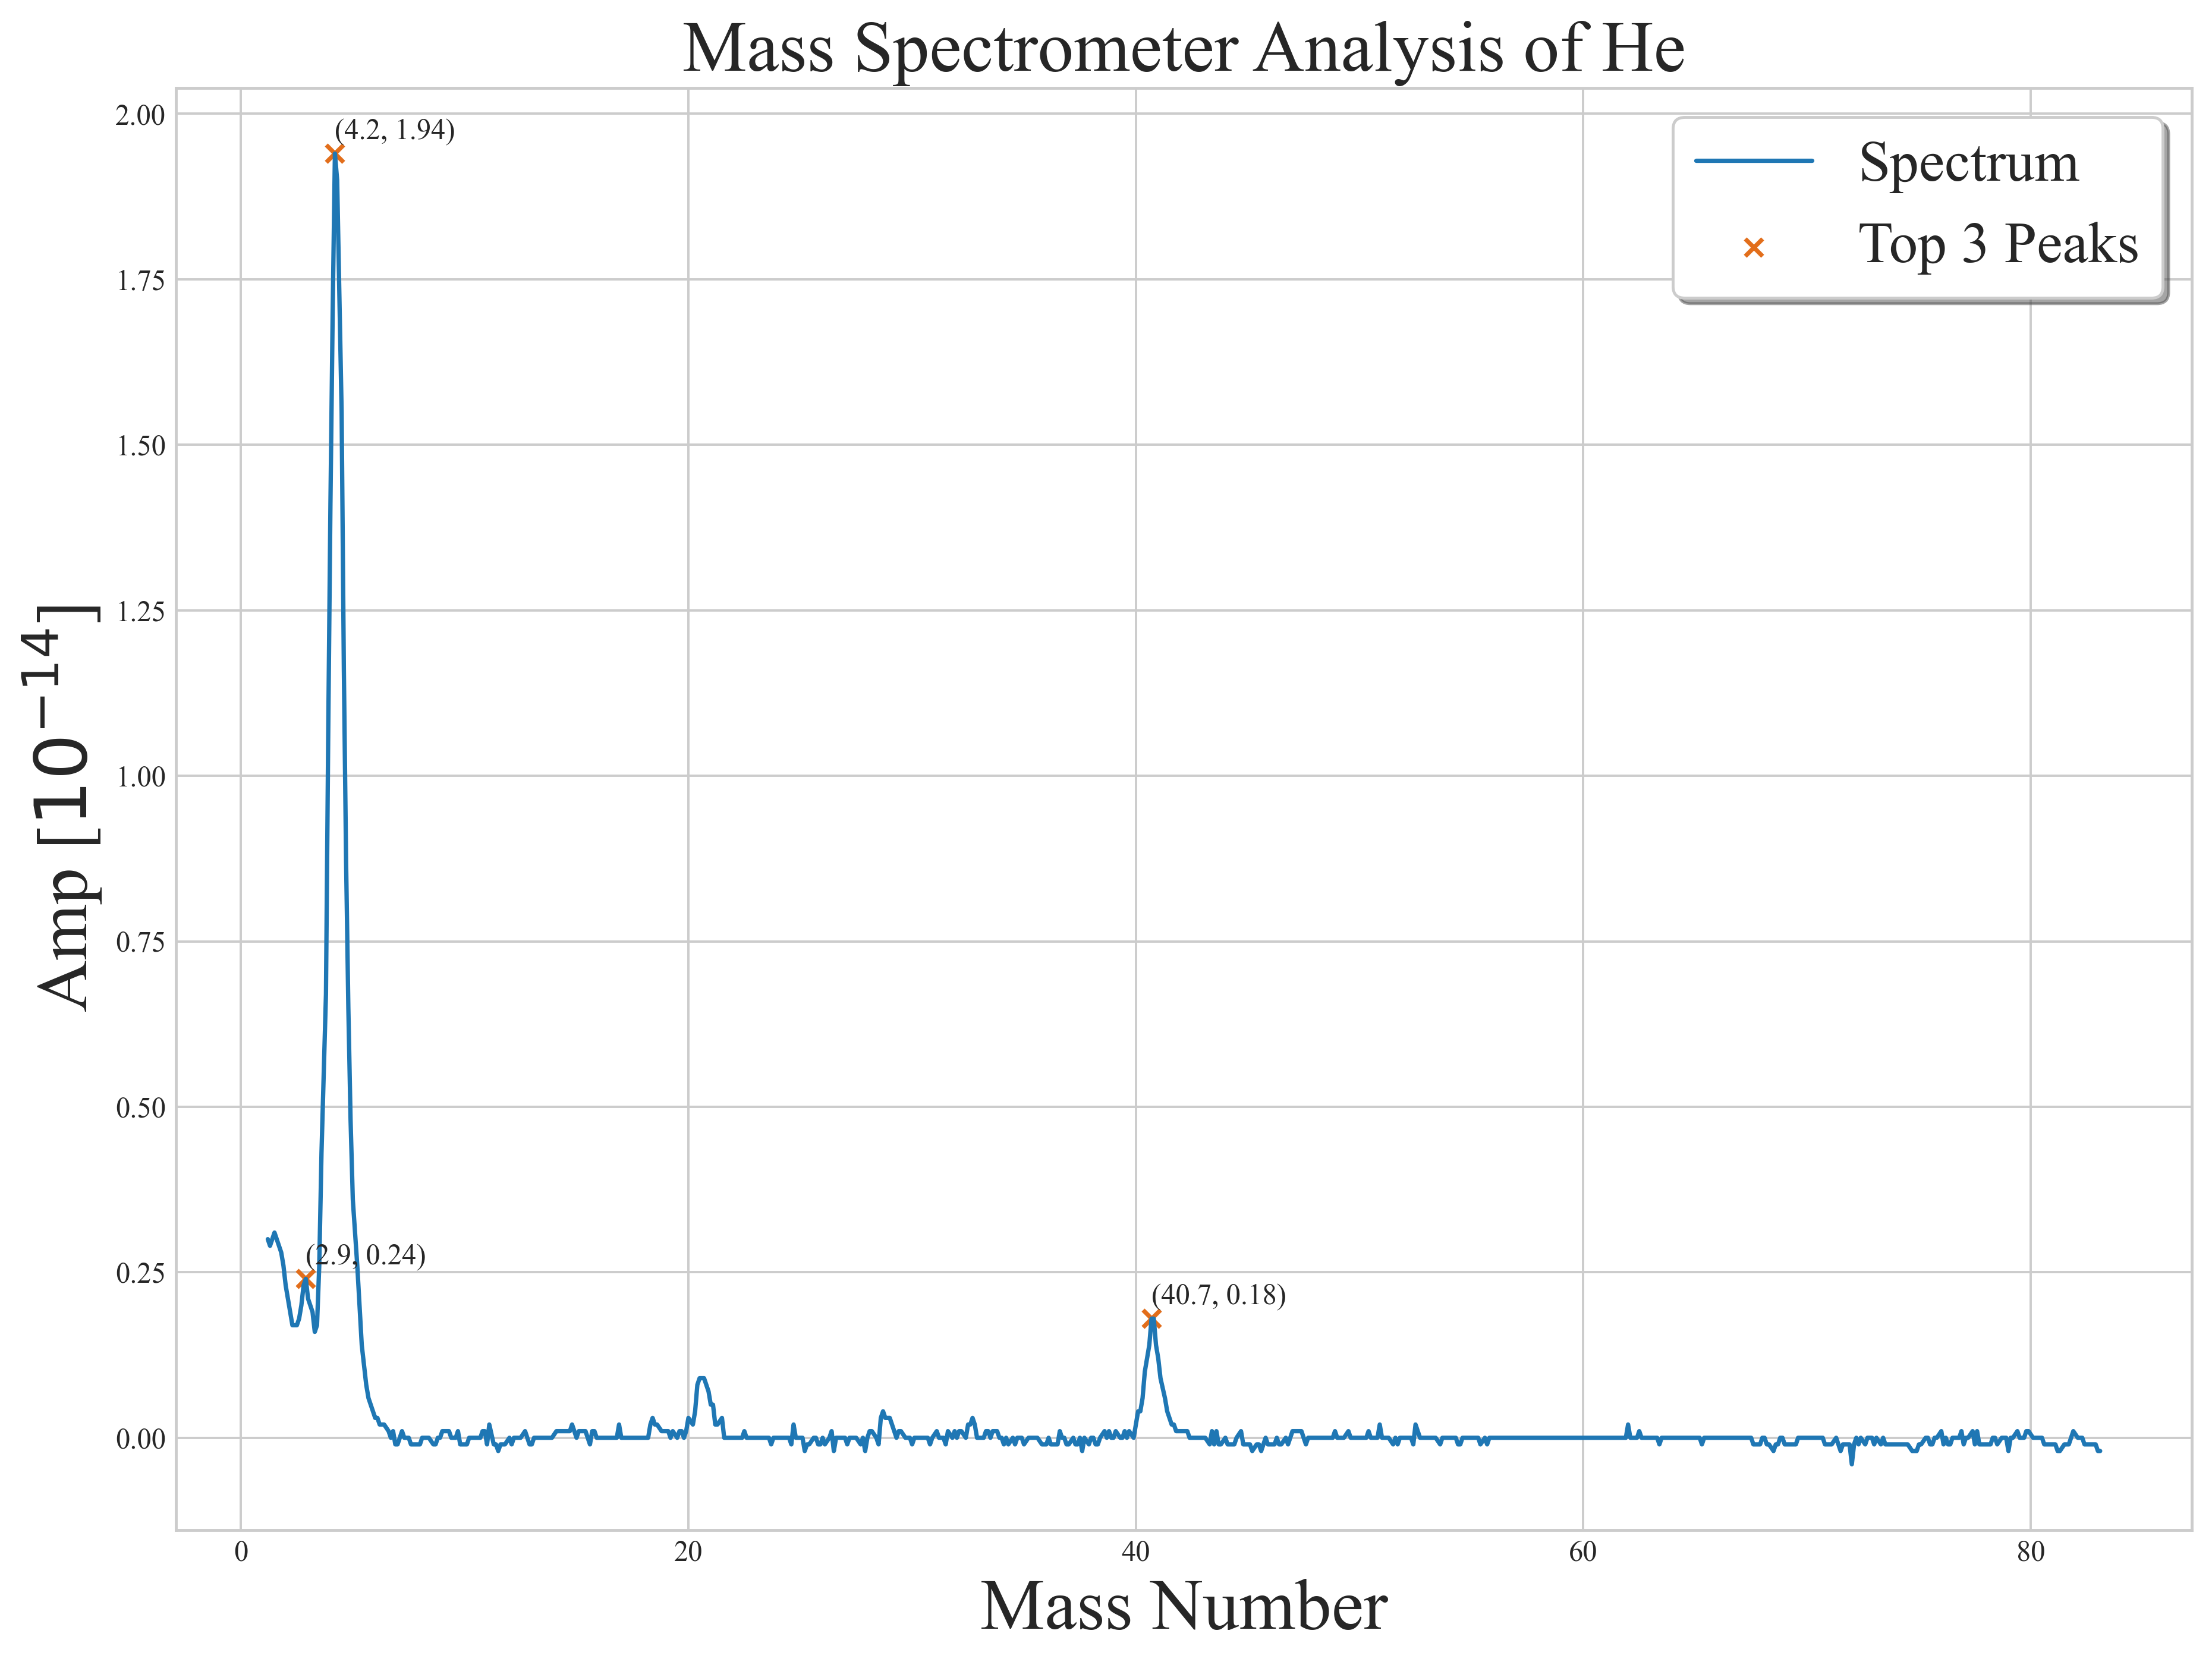
\includegraphics[width=0.7\linewidth]{images/APL1_2_4_He}
			\caption{He的质谱仪谱线分析}
			\label{fig:apl124he}
		\end{figure}
		
		\item Ne
		\begin{itemize}
			\item 质量数 20.6（主要峰）：这是 20Ne 的离子峰，对应氖气的主要同位素，约占 90.48\%。该峰是谱图中最显著的，符合高纯度氖气的主要特征。
			
			\item 质量数 22.7（次峰，未标出）：可能是 22Ne 的离子峰，22Ne 是氖气的次要同位素，约占 9.25\%。
			强度通常较主峰（20Ne）小，但应能分辨。
			
			\item 质量数 14.3 和 28.7：14.3：可能是 N+（氮离子），说明实验环境中可能有少量残余氮气。28.7：可能是 N2+（氮气分子离子） 或背景中空气的贡献。

			谱图中噪声较多，可能与真空系统中的其他气体污染有关，如空气中的氧气、氩气等。
		\end{itemize}
		
		\begin{figure}[htbp]
			\centering
			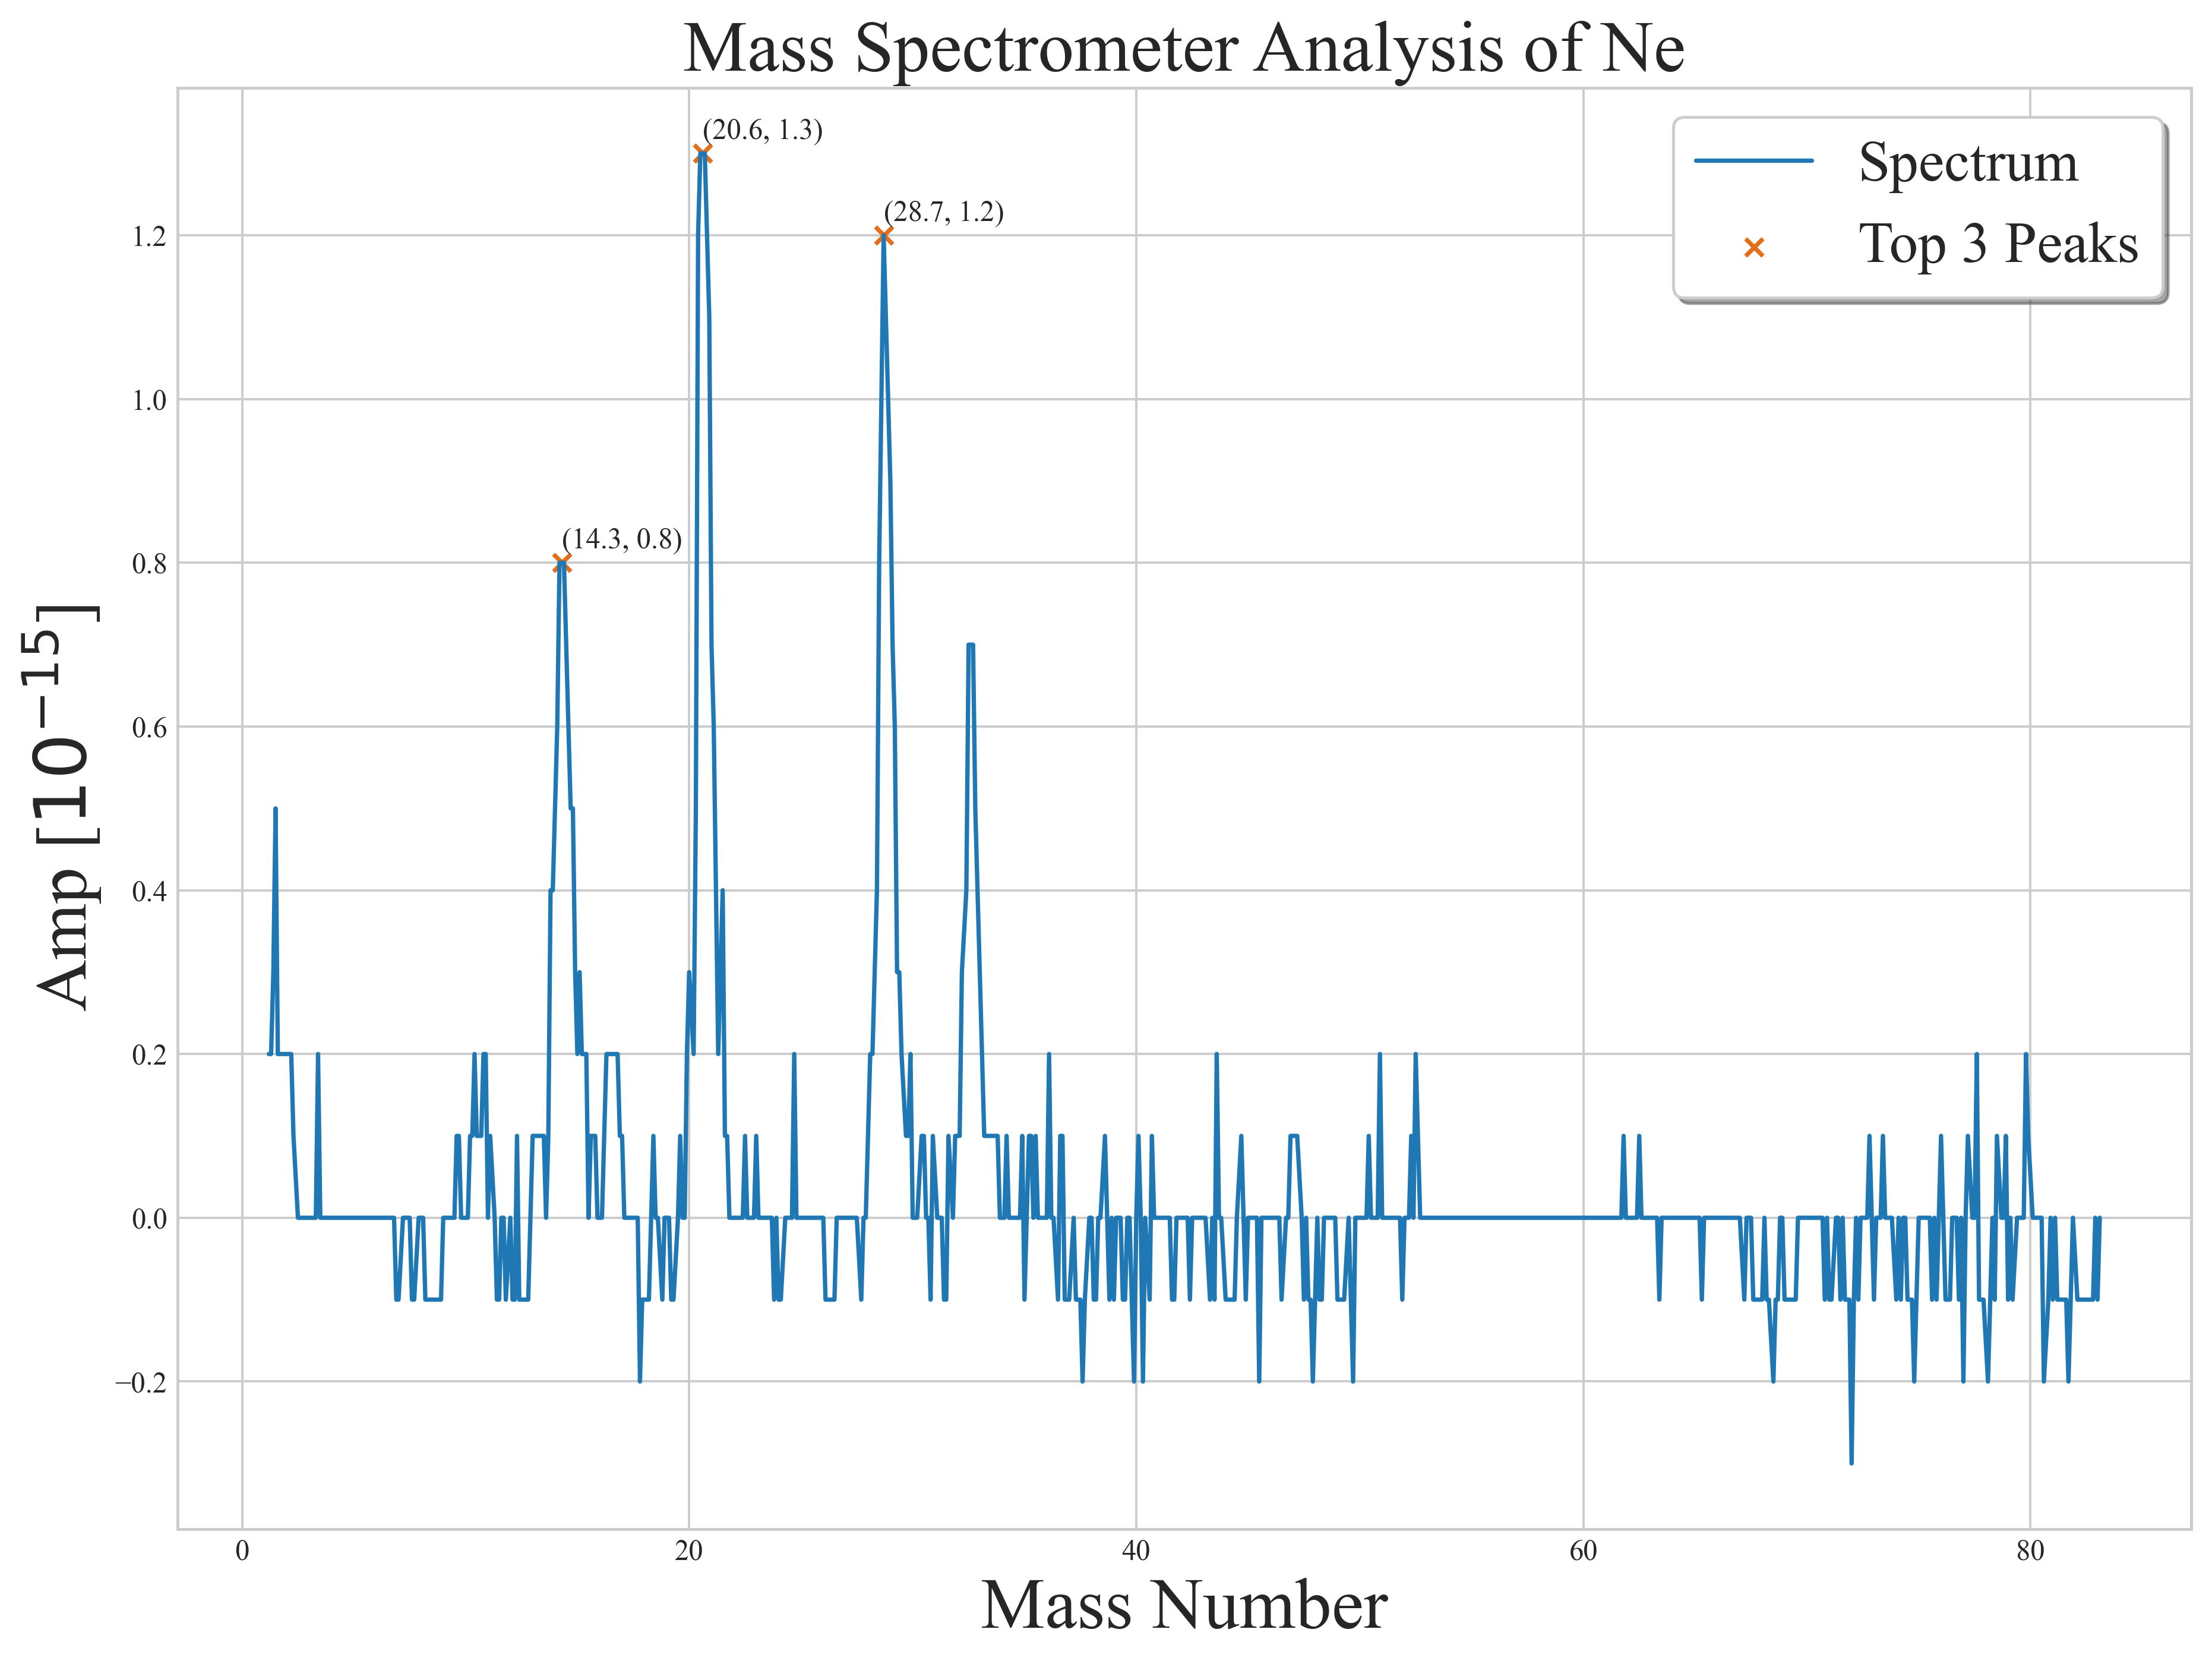
\includegraphics[width=0.7\linewidth]{images/APL1_2_4_Ne}
			\caption{Ne的质谱仪谱线分析}
			\label{fig:apl124ne}
		\end{figure}
		
	\end{enumerate}
\end{enumerate}

%% 总结
%\subsubsection{Conclusion}
%\begin{itemize}
%	\item 
%\end{itemize}


%---------------------------------------------------------------------
% 实验后思考题
\subsection{Reflections after Experiment}

%思考题1
\begin{question}
	真空度（真空计压强） 随时间变化反映了真空系统的什么特性？
\end{question}
真空度（真空计压强）随时间的变化能够反映真空系统的多个关键特性，是评估真空性能的重要指标之一。首先，真空度的变化直接体现了真空泵的抽气性能。初始阶段，真空度下降的速度越快，说明真空泵的抽气速率较高，系统排气效率较好。而在接近极限真空时，真空度下降变缓，反映了真空泵在高真空状态下的极限能力和稳定性。这一过程有助于判断真空泵的性能是否符合系统需求。

随着时间推移，真空度达到一定值后可能出现缓慢回升或波动，这通常是系统漏气或材料放气的表现。如果真空度呈线性回升，可能是密封件或法兰接口存在漏气问题；如果真空度在某个范围内波动，则可能是腔体壁或材料表面吸附的气体逐渐释放。材料的放气特性在真空度变化中也起到了重要作用，尤其是在抽气初期，吸附气体的解吸过程会减缓真空度的下降速度。当放气速率与抽气速率趋于平衡时，系统真空度会稳定在某一值，这时可以评估系统材料的洁净度和气体释放速率。

真空系统的极限真空，即最低达到的压强，体现了系统的综合性能，包括真空泵的能力、密封件的可靠性以及材料的洁净度。如果极限真空较低，说明系统的整体真空性能较优；反之，则可能需要检查密封件或腔体清洁程度。此外，在气体动态引入或调整真空系统参数时，真空度随时间的响应速度可以反映系统的动态特性。响应速度较快的系统通常表明气体流路设计合理；而响应较慢则可能受到管道阻力或死体积效应的影响。

通过记录真空度随时间的变化并进行分析，可以全面了解真空系统的性能。这不仅能够评估真空泵和系统的稳定性，还能诊断可能存在的漏气或放气问题，确保系统在实验前达到最佳状态。同时，这些数据还可以用于预测真空系统达到稳定状态所需的时间，为复杂实验的准备和运行提供可靠依据。

详见原理概述部分。

% 思考题2
\begin{question}
	等离子体光谱反映了等离子体的什么特性？ 能得到等离子体的什么参数？
\end{question}
等离子体光谱反映了等离子体的多种物理特性，是研究等离子体状态的重要工具。首先，光谱直接反映了等离子体的成分特性。通过光谱线的波长，可以识别等离子体中存在的原子、离子及分子种类，从而确定其化学组成。同时，不同谱线的强度和位置反映了粒子的激发状态和能级分布，揭示了等离子体的能量传输特性。此外，光谱的分布还可以判断等离子体是否处于局部热力学平衡 (LTE)，即粒子的激发和电离是否遵循玻尔兹曼分布和萨哈平衡。

利用等离子体光谱，可以获得多种关键参数。首先，通过分析谱线强度比，特别是不同能级跃迁的强度比，可以计算电子温度 (\(T_e\))，这一参数描述了自由电子的平均能量，是等离子体的重要热力学特性。其次，通过谱线的斯塔克加宽，可以推算电子密度 (\(n_e\))，这一参数反映了等离子体中自由电子的浓度。此外，通过综合光谱数据，结合电离平衡条件，可以进一步推算离子密度 (\(n_i\)) 和粒子间的相对丰度。

光谱的形状和宽度还可以提供有关等离子体动力学特性的信息。例如，谱线的多普勒加宽反映了粒子的热运动速度，而斯塔克加宽则与局部的电场强度和电子密度相关。结合这些信息，可以全面了解等离子体的局部微观状态，包括粒子的碰撞和能量交换机制。此外，通过分析连续光谱（自由-自由辐射和自由-束缚辐射），可以提取等离子体的光学厚度和辐射特性，为研究能量输运和电磁波与等离子体相互作用提供基础。

详见原理概述部分。

% 思考题3
\begin{question}
	研究四极电场特性及其中离子运动方程， 深入探讨四极质谱仪工作原理。
\end{question}
四极电场由四根平行排列的金属电极组成，这些电极形成了一个对称的正方形结构。通过施加交流电压和直流电压的组合，可以在空间中产生特定分布的电场，其电势分布为 \(\Phi(x, y, t) = \frac{U + V \cos(\omega t)}{r_0^2} (x^2 - y^2)\)，其中 \(U\) 是直流电压，\(V\) 是交流电压的幅值，\(\omega = 2 \pi f\) 是交流电压的角频率，\(r_0\) 是电极中心到表面的距离。这一分布产生的电场仅在 \(x\) 和 \(y\) 平面内具有分量，对离子运动施加周期性的力，而在 \(z\)-方向没有电场分量。

离子在四极电场中的运动遵循牛顿第二定律，其在 \(x\) 和 \(y\) 方向的运动方程分别为 \(\frac{d^2x}{dt^2} + \frac{q}{m} \frac{U + V \cos(\omega t)}{r_0^2} x = 0\) 和 \(\frac{d^2y}{dt^2} - \frac{q}{m} \frac{U + V \cos(\omega t)}{r_0^2} y = 0\)。这些方程为标准的 Mathieu 方程，解的稳定性决定了离子是否能够在四极电场中被传输或偏转。Mathieu 方程的一般形式为 \(\frac{d^2u}{d\xi^2} + \left[a - 2q \cos(2\xi)\right] u = 0\)，其中参数 \(a\) 和 \(q\) 的具体表达式为 \(a_x = \frac{4qU}{m \omega^2 r_0^2}\)，\(q_x = \frac{2qV}{m \omega^2 r_0^2}\)，而在 \(y\) 方向的对应值为负。通过分析 Mathieu 方程的稳定性解，可以确定离子在 \(x\) 和 \(y\) 方向的稳定区域。只有在两个方向均稳定的离子才能通过四极电场。

基于上述原理，四极质谱仪通过调整 \(U\) 和 \(V\) 的值来筛选离子质量。当 \(U/V\) 比固定时，离子的质量与电场的稳定区域直接相关，只有满足稳定性条件的离子才能通过四极电场，其它离子则会因运动不稳定而撞击电极，无法到达检测器。通过调节 \(U\) 和 \(V\) 的幅值，质谱仪可以扫描不同质量的离子。在定频模式下，保持交流频率 \(\omega\) 不变，通过调整 \(U\) 和 \(V\) 的比例选择目标质量离子。而在扫描模式下，逐步改变电压参数，使得不同质量的离子依次进入稳定区域并被检测。

离子在四极电场中的稳定性不仅取决于电场参数，还受电极几何和离子初始条件的影响。分辨率由电压调控精度、电场对称性和离子稳定区域宽度决定。灵敏度则与检测器效率、电场稳定性和离子信号强度密切相关。高分辨率要求精确的电压控制，而高灵敏度则依赖于优化的信号检测和电场设计。

详见原理概述部分。
